\begingroup
\setlength{\abovedisplayskip}{6pt}
\setlength{\belowdisplayskip}{6pt}
\setlength{\abovedisplayshortskip}{3pt}
\setlength{\belowdisplayshortskip}{4pt}

% Printed 102; principal PDF 109; Google PDF 113.
\par\clearpage
\noindent\makebox[12mm][l]{\fontsize{13}{16}\selectfont 102}\makebox[\dimexpr\linewidth-24mm\relax][c]{\footnotesize\textbf{BRIEFWECHSEL.\quad ÄNDERUNG DER POLHÖHE MIT DER HÖHE.}}\makebox[12mm][r]{}\par\medskip

\[
\theta=\frac{g'-g}{g}=\tfrac54\frac hg
\]
\noindent wird (die \textsc{Newton}sche Abplattung).

Bei dieser neuen umfassenden Form wird, wenn ich mit \textsc{Sabine}
\[
\frac{g'-g}{g}=\frac1{192{,}7}
\]
\noindent setze, die Polhöhe in \(a\)
\[
=\varphi+1070''\,.\,\frac{s}{a_0}\sin 2\varphi.
\]

Also für die höchsten Berge in Schlesien nur etwa \(\tfrac14\) Secunde. Ich muss
Ihnen indessen offenherzig gestehen, dass ich die ganze Untersuchung nur wie
eine theoretische Curiosität betrachten kann, der durchaus alle praktische Bedeutung
abgeht. Sie hätte eine solche nur dann, wenn auf der glatten Erdoberfläche
\(DAE\) eine dünne hohe Säule \(Aa\) errichtet wäre, auf deren Gipfel
wie am Fuss man die Polhöhe beobachten könnte. In der Wirklichkeit, wo
\(a\) etwa auf einem hohen Berge liegt, kann man erstlich dem Punkt \(A\) gar
nicht beikommen, und wenn man es auch könnte, und die Ungleichheit der
Richtung der Lothlinie in \(A\) und \(a\) durch Messungen scharf bestimmen
könnte, so hätte man doch gar kein Recht, obige Formel wie diesen Unterschied
darstellend zu betrachten, da die Anziehungen der oberhalb des
Niveaus von \(A\) liegenden Bestandtheile des Erdkörpers viel grössere und
einem Calcül gar nicht zu unterwerfende Ungleichheiten in den Endresultaten
für die Schwere in \(A\) und \(a\) hervorbringen werden.

Ich habe mich über diesen Gegenstand im Allgemeinen in meiner Schrift
von 1828 über den Breitenunterschied von Göttingen und Altona, p.~73 [vergl.\
diesen Band, S.~49], bereits so ausgesprochen, dass ich jetzt nichts Besseres
darüber zu sagen weiss.

\begin{center}\rule{.18\textwidth}{.4pt}\end{center}
{\small
\begin{center}\textbf{BEMERKUNGEN.}\end{center}
Der vorstehende Brief, von dem eine Abschrift im Gauss-Archiv vorhanden ist, ist abgedruckt in den
»Protocollen der Verhandlungen der permanenten Commission der europäischen Gradmessung vom 23. bis
29. September 1869 in Florenz«. (Als Manuscript gedruckt.) S.~30---32.
\par\hfill\textsc{Krüger, Börsch.}\hspace{.06\textwidth}\par
}
\begin{center}\rule{.24\textwidth}{.4pt}\end{center}

% Printed 103; principal PDF 110; Google PDF 114.
\par\clearpage

\vspace*{.09\textheight}
\begin{center}{\LARGE N\,A\,C\,H\,L\,A\,S\,S.}\end{center}
\vspace{.05\textheight}
\begin{center}
[1.]\\[.5ex]
Reduction der sphärischen Dreieckswinkel \(A,B,C\) auf die Chordenwinkel\\
\(\mathfrak{A},\mathfrak{B},\mathfrak{C}\).
\end{center}

\noindent\begin{minipage}[t]{.65\textwidth}
\setlength{\parindent}{1.5em}
\indent Man beschreibe um das Dreieck einen Kreis.\\
Also die 3 Vierecke das Maass [der Correctionen].

Man mache
\[
\frac{a}{\sin A}=\frac{b}{\sin B}=\frac{c}{\sin C}=\nu
\]
\[
\nu a\cos A=\alpha,\quad \nu b\cos B=\beta,\quad \nu c\cos C=\gamma.
\]
\noindent Dann sind die Reductionen
\[
\frac{\beta+\gamma}{8},\quad
\frac{\alpha+\gamma}{8},\quad
\frac{\alpha+\beta}{8}.
\]
\end{minipage}\hfill
\begin{minipage}[t]{.33\textwidth}
\vspace{0pt}\centering
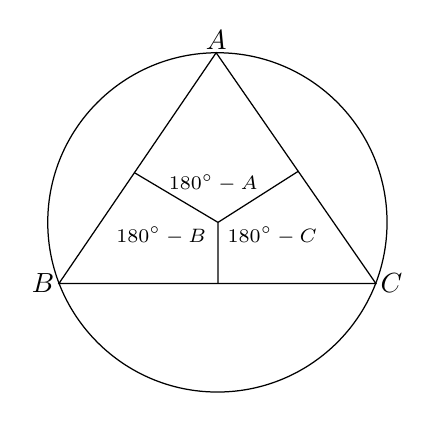
\begin{tikzpicture}[x=1.55cm,y=1.55cm,line width=.45pt]
\coordinate (A) at (-.01,1.39);
\coordinate (B) at (-1.298,-.50);
\coordinate (C) at (1.298,-.50);
\coordinate (O) at (.005,0);
\path (A)--(B) coordinate[pos=.52] (AB);
\path (A)--(C) coordinate[pos=.514] (AC);
\path (B)--(C) coordinate[pos=.502] (BC);
\draw (0,0) circle[radius=1.39];
\draw (A)--(B)--(C)--cycle;
\draw (AB)--(O)--(AC) (O)--(BC);
\node[above,inner sep=1pt] at (A) {\(A\)};
\node[left,inner sep=1.5pt] at (B) {\(B\)};
\node[right,inner sep=1.5pt] at (C) {\(C\)};
\node[font=\scriptsize,inner sep=0pt] at (-.035,.32) {\(180^\circ-\mathfrak A\)};
\node[font=\scriptsize,inner sep=0pt] at (-.46,-.11) {\(180^\circ-\mathfrak B\)};
\node[font=\scriptsize,inner sep=0pt] at (.45,-.11) {\(180^\circ-\mathfrak C\)};
\end{tikzpicture}
\end{minipage}
\par\bigskip

\begin{center}
[2.]\\[.5ex]
{[Bedingung dafür, dass 3 Punkte auf der Oberfläche einer Kugel}\\
auf einem grössten Kreise liegen.]
\end{center}

Dass drei Punkte auf der Oberfläche einer Kugel, deren Längen und
Breiten resp.
\[
\begin{array}{l}
L,\ B\\
L',\ B'\\
L'',\ B''
\end{array}
\]
\noindent sind, in einem grössten Kreise liegen, davon ist die Bedingungsgleichung:
\[
\operatorname{tang}B\sin(L'-L'')+\operatorname{tang}B'\sin(L''-L)+
\operatorname{tang}B''\sin(L-L')=0.
\]

\begin{center}\rule{.18\textwidth}{.4pt}\end{center}

% Printed 104; principal PDF 111; Google PDF 115.
\par\clearpage
\noindent\makebox[12mm][l]{\fontsize{13}{16}\selectfont 104}\makebox[\dimexpr\linewidth-24mm\relax][c]{\scriptsize\textbf{BEMERKUNGEN.\quad REDUCTION DER SPHÄRISCHEN DREIECKSWINKEL ETC.}}\makebox[12mm][r]{}\par\medskip

\vspace*{.11\textheight}
{\small
\begin{center}\textbf{BEMERKUNGEN.}\end{center}

Die Notiz [1] ist in ein Rechnungsheft für die hannoversche Gradmessung eingetragen. \textsc{Gauss} hat
hier als Werthe der Correctionen \(\frac{\beta+\gamma}{4}\), \(\frac{\alpha+\gamma}{4}\), \(\frac{\alpha+\beta}{4}\) angegeben. Die Reduction von \(A\) auf \(\mathfrak A\) kann man
aus der Gleichung
\[
\cos\mathfrak A=\sin\frac b{2r}\sin\frac c{2r}
+\cos\frac b{2r}\cos\frac c{2r}\cos A,\quad (r=\text{Radius der Kugel})
\]
\noindent erhalten, die entwickelt zunächst
\[
A-\mathfrak A=\frac1{4rr}\,.\,\frac{bc}{\sin A}
-\frac1{8rr}(bb+cc)\operatorname{cotang}A\ldots
\]
\noindent liefert. Beschränkt man sich auf die Glieder zweiter Ordnung, so kann man
\[
bb+cc=aa+2bc\cos A
\]
\noindent setzen. Damit ergibt sich
\[
A-\mathfrak A=\frac1{8rr}(2bc\sin A-aa\operatorname{cotang}A)
=\frac1{8rr}(bb\operatorname{cotang}B+cc\operatorname{cotang}C).
\]
\noindent Zu demselben Ergebniss gelangt man, wenn man bedenkt, dass \(A-\mathfrak A\) gleich dem Excesse des sphärischen
Vierecks ist, dessen Eckpunkte der Pol des Dreiecks, die Fusspunkte der Lothe von diesem auf die Seiten
\(b\) und \(c\) und der Punkt \(A\) sind.

Die Notiz [2] befindet sich auf dem letzten Blatte des \textsc{Gauss}schen Exemplars der »Analytischen
Trigonometrie von G. S. \textsc{Klügel}. Braunschweig 1770«. Nach einer von \textsc{Gauss} gehaltenen Vorlesung:
»Anleitung zur höhern Geodäsie«, von der eine Nachschrift vorliegt, gründet sich die Ableitung der in [2]
gegebenen Bedingungsgleichung darauf, dass, wenn
\[
\begin{aligned}
m&=n\sin(\varphi-\Phi)\\
m'&=n\sin(\varphi'-\Phi)\\
m''&=n\sin(\varphi''-\Phi)
\end{aligned}
\]
\noindent ist, alsdann
\[
m\sin(\varphi'-\varphi'')+m'\sin(\varphi''-\varphi)+m''\sin(\varphi-\varphi')=0
\]
\noindent wird. Bedeutet nun \(i\) den Neigungswinkel der Ebene des grössten Kreises gegen die Äquatorebene, und
werden die Längen \(L-L_0\), \(L'-L_0\), \(L''-L_0\) von dem durch den Durchschnitt beider gehenden Meridian
an gezählt, so ist aber
\[
\begin{aligned}
\operatorname{tang}B&=\operatorname{tang}i\sin(L-L_0)\\
\operatorname{tang}B'&=\operatorname{tang}i\sin(L'-L_0)\\
\operatorname{tang}B''&=\operatorname{tang}i\sin(L''-L_0).
\end{aligned}
\]
\par\hfill\textsc{Krüger, Börsch.}\hspace{.06\textwidth}\par
}
\begin{center}\rule{.24\textwidth}{.4pt}\end{center}

% Printed 105; principal PDF 112; Google PDF 116.
\par\clearpage

\thispagestyle{empty}
\vspace*{\fill}
\begin{center}
\LARGE
CONFORME DOPPELPROJECTION\\[.5ex]
DES SPHÄROIDS AUF DIE KUGEL\\[.5ex]
UND DIE EBENE.
\end{center}
\vspace*{\fill}

% Printed 106; principal PDF 113; Google PDF 117.
\par\clearpage

\thispagestyle{empty}
\null

% Printed 107; principal PDF 114; Google PDF 118.
\par\clearpage

\vspace*{.11\textheight}
\begin{center}{\LARGE N\,A\,C\,H\,L\,A\,S\,S.}\end{center}
\vspace{.05\textheight}
\begin{center}
[I.]\par\bigskip
{\Large DAS ELLIPTISCHE SPHÄROID\\
{[AUF DIE KUGEL ÜBERTRAGEN].}}\par\bigskip
\rule{.09\textwidth}{.4pt}\par\bigskip
[1.]
\end{center}

Die erste Aufgabe ist die Übertragung der Oberfläche des Ellipsoids auf
die Kugelfläche.

[Es sei]
\[
\begin{array}{l@{\;\ldotp\;\ldotp\;\ldotp\;\ldotp\;}l}
\varphi & \text{Polhöhe auf dem Sphäroid}\\
\psi & \text{correspondirende Polhöhe auf der Kugel}\\
e & \text{Excentricität}\\
a & \text{Halbmesser des Äquators.}
\end{array}
\]
\noindent [Dann ist, vergl.\ Band IV, Art.~13, S.~207 u.\ f.]
\[
\frac{\mathrm d\psi}{\cos\psi}
=\frac{(1-ee)\,\mathrm d\varphi}{\cos\varphi(1-ee\sin\varphi^2)}
\]
\noindent oder
\[
\operatorname{tang}(45^\circ+\tfrac12\psi)
=\operatorname{tang}(45^\circ+\tfrac12\varphi)
\left(\frac{1-e\sin\varphi}{1+e\sin\varphi}\right)^{\frac12 e}\,.\,\text{Const.}
\]

\noindent Jede unendlich kleine Figur auf der Kugel wird so der correspondirenden
auf dem Sphäroid ähnlich, und gleich, wenn man den Halbmesser der Kugel
\(r=\frac{a\cos\varphi}{\cos\psi\surd(1-ee\sin\varphi^2)}\) setzt. Soll \(r\) für \(\varphi=P\)
ein Maximum werden, so setzt man den constanten Multiplicator
\(=\bigl(\frac{1+e\sin P}{1-e\sin P}\bigr)^{\frac12 e}\), wodurch auf jenem Parallel
auch \(\psi=P\) wird. Man hat dann eben daselbst die vollkommenste Gleich-
\par\smallskip
\noindent\hfill \(14^{*}\)\hspace{.12\textwidth}\par

% Printed 108; principal PDF 115; Google PDF 119.
\par\clearpage
\noindent\makebox[12mm][l]{\fontsize{13}{16}\selectfont 108}\makebox[\dimexpr\linewidth-24mm\relax][c]{\small\textbf{NACHLASS.}}\makebox[12mm][r]{}\par\medskip

\noindent heit der Figuren, wenn man den Halbmesser der Kugel
\(=\frac a{\surd(1-ee\sin P^2)}\) setzt. Für andere Parallele sind dann die Lineargrössen
auf dem Sphäroid zu denen auf der Kugel wie
\[
\frac{\cos\varphi\surd(1-ee\sin P^2)}{\cos\psi\surd(1-ee\sin\varphi^2)}:1=1:n.
\]

\noindent [Hieraus folgt
\[
\frac{\mathrm d\log n}{\mathrm d\psi}=\Big]
\frac{\mathrm dn}{n\,\mathrm d\psi}=\frac{\sin\varphi-\sin\psi}{\cos\psi}.
\]

\noindent Die Darstellung eines Stückes der geodätischen Linie auf der Kugel wird
hier ein kleiner Kreis; setzt man dessen Radius \(=R\), so ist
\[
\operatorname{cotang} R=\frac{\sin\varphi-\sin\psi}{\cos\psi}\sin\zeta
\left[=\frac{\mathrm d\log n}{\mathrm d\psi}\sin\zeta\right],
\]
\noindent [wo] \(\zeta\) [das] Azimuth [der geodätischen Linie bedeutet].

[Die Darstellung ist] concav nach Süden, wenn \(\sin\varphi>\sin\psi\) ist.

\bigskip
\begin{center}[2.]\end{center}
Es sei
\[
\begin{aligned}
\sin\varphi&=s\\
\sin\psi&=\sigma,
\end{aligned}
\]
\noindent [also]
\[
\begin{aligned}
\frac{\mathrm ds}{\mathrm d\sigma}
&=\frac{(1-eess)(1-ss)}{(1-ee)(1-\sigma\sigma)}
=\frac{1-(1+ee)ss+ees^4}{(1-ee)(1-\sigma\sigma)}\\
\frac{\mathrm{dd}s}{\mathrm d\sigma^2}
&=\frac{(1-eess)(1-ss)}{(1-ee)^2(1-\sigma\sigma)^2}
\{(2-2ee)\sigma-(2+2ee)s+4ees^3\}
\end{aligned}
\]
\noindent\hfill u.\ s.\ w.\hfill\null\par

\noindent Für [\(\varphi=\)] \(\psi=P\) werden diese Werthe:
\[
\begin{aligned}
\frac{\mathrm ds}{\mathrm d\sigma}
&=\frac{1-ee\sin P^2}{1-ee}\\
\frac{\mathrm{dd}s}{\mathrm d\sigma^2}
&=-\frac{4ee}{(1-ee)^2}(1-ee\sin P^2)\sin P\\
\mathopen{\Big[}\frac{\mathrm d^3s}{\mathrm d\sigma^3}
&=-2ee\frac{1-ee\sin P^2}{(1-ee)^3\cos P^2}
\{3-ee-(3+13ee)\sin P^2+14ee\sin P^4\}\Big].
\end{aligned}
\]
\noindent Folglich
\[
\sin\varphi=\sin P+\frac{1-ee\sin P^2}{1-ee}(\sin\psi-\sin P)
-\frac{2ee}{(1-ee)^2}(1-ee\sin P^2)\sin P(\sin\psi-\sin P)^2-\ldots
\]

% Printed 109; principal PDF 116; Google PDF 120.
\par\clearpage
\noindent\makebox[12mm][l]{}\makebox[\dimexpr\linewidth-24mm\relax][c]{\footnotesize\textbf{CONFORME PROJECTION DES SPHÄROIDS AUF DIE KUGEL.}}\makebox[12mm][r]{\fontsize{13}{16}\selectfont 109}\par\medskip

\noindent [oder]
\[
\begin{gathered}
\sin\varphi-\sin\psi=\frac{ee\cos P^2}{1-ee}(\sin\psi-\sin P)
-\frac{2ee}{(1-ee)^2}(1-ee\sin P^2)\sin P(\sin\psi-\sin P)^2\\
-\left[\frac{ee}{3(1-ee)^3}\,.\,\frac{1-ee\sin P^2}{\cos P^2}
\{3-ee-(3+13ee)\sin P^2+14ee\sin P^4\}(\sin\psi-\sin P)^3\right]\ldots.
\end{gathered}
\]
\noindent Ferner ist
\[
\cos\psi^2=\cos P^2-2\sin P(\sin\psi-\sin P)-[(\sin\psi-\sin P)^2].
\]
\noindent Also
\[
\begin{aligned}
&\frac{\mathrm d\log n}{\mathrm d\sin\psi}
\left[=\frac{\sin\varphi-\sin\psi}{\cos\psi^2}\right]\\
&=\frac{ee}{1-ee}(\sin\psi-\sin P)-\frac{2e^4\sin P}{(1-ee)^2}(\sin\psi-\sin P)^2
-\frac{e^4(5-ee(3+14\sin P^2))}{3(1-ee)^3}(\sin\psi-\sin P)^3\ldots
\end{aligned}
\]
\noindent und
\[
\begin{aligned}
\log n
&=\frac{ee}{2(1-ee)}(\sin\psi-\sin P)^2
-\frac{2e^4\sin P}{3(1-ee)^2}(\sin\psi-\sin P)^3\ldots\\
&=\alpha(\sin\psi-\sin P)^2-\beta(\sin\psi-\sin P)^3\ldots.
\end{aligned}
\]
\noindent [Für den Abplattungswerth \(\frac1{303{,}45..}\) und \(P=51^\circ31'48''{,}70\) ist]
\[
\begin{array}{@{}r@{\quad}l@{}}
\makebox[25mm][s]{\(\displaystyle\frac{ee}{1-ee}\)\hfill .\hfill .\hfill .\hfill .\hfill .}
&7{,}821\,0885\\[.7ex]
\makebox[25mm][s]{\(\displaystyle\frac{\mathrm{Mod.}}2\)\hfill .\hfill .\hfill .\hfill .\hfill .\hfill .}
&9{,}336\,7543\\[.7ex]\hline
\log\alpha=&7{,}157\,8428\\[.5ex]
\makebox[25mm][s]{\(\displaystyle\frac{ee}{1-ee}\)\hfill .\hfill .\hfill .\hfill .\hfill .}
&7{,}821\,0885\\[.7ex]
\makebox[25mm][s]{\(\tfrac43\)\hfill .\hfill .\hfill .\hfill .\hfill .\hfill .\hfill .\hfill .}
&0{,}124\,9387\\
\makebox[25mm][s]{\(\sin P\)\hfill .\hfill .\hfill .\hfill .\hfill .}
&9{,}893\,7263\\\hline
\log\beta=&4{,}997\,5963
\end{array}
\]
\noindent [also für briggische Logarithmen]
\[
\log n=0{,}001\,4382.78(\sin\psi-\sin P)^2-0{,}000\,0099.45(\sin\psi-\sin P)^3\ldots.
\]

\begin{center}[3.]\end{center}
Ferner ist
\[
\begin{aligned}
\frac{\mathrm ds}{\mathrm d\psi}
&=\frac{1-(1+ee)ss+ees^4}{(1-ee)\surd(1-\sigma\sigma)},\\
\frac{\mathrm{dd}s}{\mathrm d\psi^2}
&=\frac{(1-ss)(1-eess)}{(1-ee)^2(1-\sigma\sigma)}
\{(1-ee)\sigma-2(1+ee)s+4ees^3\}
\end{aligned}
\]
\noindent\hfill u.\ s.\ w.\hfill\null\par

% Printed 110; principal PDF 117; Google PDF 121.
\par\clearpage
\noindent\makebox[12mm][l]{\fontsize{13}{16}\selectfont 110}\makebox[\dimexpr\linewidth-24mm\relax][c]{\small\textbf{NACHLASS.}}\makebox[12mm][r]{}\par\medskip

\noindent Also für [\(\varphi=\)] \(\psi=P\):
\[
\begin{aligned}
\frac{\mathrm ds}{\mathrm d\psi}
&=\frac{(1-ee\sin P^2)\cos P}{1-ee}\\
\frac{\mathrm{dd}s}{\mathrm d\psi^2}
&=-\frac{(1-ee\sin P^2)\sin P}{(1-ee)^2}(1+3ee-4ee\sin P^2)\\
\mathopen{\Big[}\frac{\mathrm d^3s}{\mathrm d\psi^3}
&=-\frac{(1-ee\sin P^2)\cos P}{(1-ee)^3}
\{1+4ee-e^4-(18ee+14e^4)\sin P^2+28e^4\sin P^4\},
\end{aligned}
\]
\noindent folglich]
\[
\begin{gathered}
\sin\varphi=\sin P+\frac{(1-ee\sin P^2)\cos P}{1-ee}(\psi-P)
-\frac{(1-ee\sin P^2)\sin P}{2(1-ee)^2}(1+3ee-4ee\sin P^2)(\psi-P)^2\\
-\left[\frac{(1-ee\sin P^2)\cos P}{6(1-ee)^3}
\{1+4ee-e^4-(18ee+14e^4)\sin P^2+28e^4\sin P^4\}(\psi-P)^3\right]\ldots.
\end{gathered}
\]
\noindent [Da]
\[
\sin\psi=\sin P+\cos P\,.\,(\psi-P)-\tfrac12\sin P\,.\,(\psi-P)^2
-[\tfrac16\cos P\,.\,(\psi-P)^3]\ldots
\]
\noindent [ist, so wird]
\[
\begin{aligned}
\sin\varphi-\sin\psi&=\frac{ee\cos P^3}{1-ee}(\psi-P)\\
&\quad-\frac{ee}{2(1-ee)^2}\sin P\{5-ee-(5+3ee)\sin P^2+4ee\sin P^4\}(\psi-P)^2\\
&\quad-\Big[\frac{ee}{6(1-ee)^3}\cos P\{7-4ee+e^4-(19+18ee-e^4)\sin P^2\\
&\qquad\qquad\qquad+(46ee+14e^4)\sin P^4-28e^4\sin P^6\}(\psi-P)^3\Big]\ldots.
\end{aligned}
\]
\noindent [Mit]
\[
\cos\psi=\cos P-\sin P\,.\,(\psi-P)-[\tfrac12\cos P\,.\,(\psi-P)^2]\ldots
\]
\noindent [folgt daher]
\[
\begin{aligned}
&\frac{\mathrm d\log n}{\mathrm d\psi}
\left[=\frac{\sin\varphi-\sin\psi}{\cos\psi}\right]\\
&\quad=\frac{ee}{1-ee}\cos P^2\,.\,(\psi-P)
-\tfrac12\frac{ee}{1-ee}\sin P\cos P
\left(3+4\frac{ee}{1-ee}\cos P^2\right)(\psi-P)^2\\
&\qquad-\Big\{\frac{ee}{1-ee}(\tfrac23\cos P^2-\tfrac12\sin P^2)
-\left(\frac{ee}{1-ee}\right)^2(4\sin P^2-\tfrac53\cos P^2)\cos P^2\\
&\qquad\qquad\qquad-\left(\frac{ee}{1-ee}\right)^3
(4\sin P^2-\tfrac23\cos P^2)\cos P^4\Big\}(\psi-P)^3\ldots.
\end{aligned}
\]

% Printed 111; principal PDF 118; Google PDF 122.
\par\clearpage
\noindent\makebox[12mm][l]{}\makebox[\dimexpr\linewidth-24mm\relax][c]{\footnotesize\textbf{CONFORME PROJECTION DES SPHÄROIDS AUF DIE KUGEL.}}\makebox[12mm][r]{\fontsize{13}{16}\selectfont 111}\par\medskip

\begin{center}[4.]\end{center}
[Man setze
\[
\psi-P=\frac{x\surd(1-ee\sin P^2)}a
\]
\noindent und]
\[
\frac{ee}{1-ee}=h;
\]
\noindent \(x\) [sei] nach Süden positiv.\quad [Dann wird]
\[
\begin{aligned}
\log n&=\tfrac12h\cos P^2\,\frac{xx(1-ee\sin P^2)}{aa}\\
&\quad+\tfrac12h\sin P\cos P(1+\tfrac43h\cos P^2)
\frac{x^3(1-ee\sin P^2)^{\frac32}}{a^3}\\
&\quad-\{h(\tfrac16\cos P^2-\tfrac18\sin P^2)
-hh(\sin P^2-\tfrac5{12}\cos P^2)\cos P^2\\
&\qquad\qquad-h^3(\sin P^2-\tfrac16\cos P^2)\cos P^4\}
\frac{x^4(1-ee\sin P^2)^2}{a^4}
\end{aligned}
\]
\noindent\hfill etc.\hfill\null\par

\bigskip
\begin{center}[5.]\end{center}
[Ist \(\xi\) der dem \(x\) entsprechende Werth auf dem Sphäroid, so ist
\[
\frac{\mathrm d\xi}{\mathrm dx}=\frac1n=1-\log n+\tfrac12(\log n)^2\ldots,
\]
\noindent also, wenn noch]
\[
r=\frac a{\surd(1-ee\sin P^2)}
\]
\noindent [gesetzt wird:]
\[
\xi=x-\alpha x^3-\beta x^4+\gamma x^5\ldots;
\]
\[
\begin{aligned}
\alpha&=\frac{h\cos P^2}{6rr}\\
\beta&=\frac{h\sin P\cos P}{8r^3}(1+\tfrac43h\cos P^2)\\
\gamma&=\frac1{r^4}\{h(\tfrac1{30}\cos P^2-\tfrac1{40}\sin P^2)
-hh(\tfrac15\sin P^2-\tfrac{13}{120}\cos P^2)\cos P^2\\
&\qquad\qquad-h^3(\tfrac15\sin P^2-\tfrac1{30}\cos P^2)\cos P^4\}.
\end{aligned}
\]
\par
\endgroup
